\documentclass[12pt]{article}
\usepackage{graphicx}
\usepackage[none]{hyphenat}
\usepackage{graphicx}
\usepackage{listings}
\usepackage[english]{babel}
\usepackage{graphicx}
\usepackage{caption} 
\usepackage{booktabs}
\usepackage{array}
\usepackage{amssymb} % for \because
\usepackage{amsmath}   % for having text in math mode
\usepackage{extarrows} % for Row operations arrows
\usepackage{listings}
\lstset{
  frame=single,
  breaklines=true
}
\usepackage{hyperref}
\usepackage{bm}
  
%Following 2 lines were added to remove the blank page at the beginning
\usepackage{atbegshi}% http://ctan.org/pkg/atbegshi
\AtBeginDocument{\AtBeginShipoutNext{\AtBeginShipoutDiscard}}
\usepackage{gensymb}


%New macro definitions
\newcommand{\mydet}[1]{\ensuremath{\begin{vmatrix}#1\end{vmatrix}}}
\providecommand{\brak}[1]{\ensuremath{\left(#1\right)}}
\providecommand{\sbrak}[1]{\ensuremath{{}\left[#1\right]}}
\providecommand{\norm}[1]{\left\lVert#1\right\rVert}
\providecommand{\abs}[1]{\left\vert#1\right\vert}
\newcommand{\solution}{\noindent \textbf{Solution: }}
\newcommand{\myvec}[1]{\ensuremath{\begin{pmatrix}#1\end{pmatrix}}}
\let\vec\mathbf


\begin{document}

\begin{center}
\title{\textbf{3D Lines}}
\date{\vspace{-5ex}} %Not to print date automatically
\maketitle
\end{center}
\setcounter{page}{1}

\section{JEE Maths - 65 C-1}
This is Problem-30 
\begin{enumerate}
\item Find the shortest distance between the lines $\frac{x-1}{2} = \frac{y+1}{3}=z$ and $\frac{x+1}{5} = \frac{y-2}{1}; z=2 $ 

\solution 
The given equation can be written as
\begin{align}
	\frac{x-1}{2} &= \frac{y+1}{3}=\frac{z-0}{1}\\ 
	\frac{x+1}{5} &= \frac{y-2}{1}= \frac{z-2}{0} \\ 
	\implies 
	\vec{A} &= \vec{x}_1 + \lambda_1\vec{m}_1\\
	\vec{B} &= \vec{x}_2 + \lambda_2\vec{m}_2
\end{align}	
where
\begin{align}
	&\vec{x_1} = \myvec{1\\-1\\0},  
	\vec{x_2} = \myvec{-1\\2\\2},  
	\vec{m_1} = \myvec{2\\3\\1},
	\vec{m_2} = \myvec{5\\1\\0}  
\end{align}	
Assume
\begin{align}
	&\vec{M} = \myvec{\vec{m}_1 & \vec{m}_2} 
\end{align}
\begin{align}
	&\vec{B}-\vec{A} = \brak{\lambda_2\vec{m}_2 - \lambda_1\vec{m}_1} + \brak{\vec{x}_2- \vec{x}_1} \\ 
	\label{eq:Eq1}
	&= \vec{M}\bm{\lambda}+ \vec{k} \\
	\text{ where } \bm{\lambda} &\triangleq \myvec{-\lambda_1\\ \lambda_2}\text{ and }\vec{k} =\brak{\vec{x}_2- \vec{x}_1}  \\
\end{align}
We can formulate an unconstrained optimization problem as below:
\begin{align}
	\label{eq:Eq2}
	&  \min_{\bm{\lambda}} \quad \norm{\vec{B}-\vec{A}}^2 
\end{align}
Substituting \eqref{eq:Eq1} in \eqref{eq:Eq2}
\begin{align}
	\eqref{eq:Eq2} \implies 
	&  \min_{\bm{\lambda}} \quad \norm{\vec{M}\bm{\lambda}+\vec{k}}^2 \\ 
	&\implies \text{f}\brak{\bm{\lambda}} = \brak{\vec{M}\bm{\lambda}+\vec{k}}^\top\brak{\vec{M}\bm{\lambda}+\vec{k}} \\
	&= \brak{\bm{\lambda}^\top\vec{M}^\top+\vec{k}^\top}\brak{\vec{M}\bm{\lambda}+\vec{k}} \\
	\label{eq:Eq4} 
	&= \bm{\lambda}^\top\vec{M}^\top\vec{M}\bm{\lambda}+2\vec{M}\bm{\lambda}\vec{k}^\top+ \norm{\vec{k}}^2 
\end{align}
Equation \eqref{eq:Eq4} is a quadratric vector equation. To check whether it is convex or not, we will compute the value of $\vec{M}^\top\vec{M}$.
\begin{align}
	&\vec{M}^\top\vec{M} =  \myvec{2&3&1\\5&1&0}\myvec{2&5\\3&1\\1&0} = \myvec{14&13\\13&26}
\end{align}
The eigen values of $\vec{M}^\top\vec{M}$ are $34.73$ and $5.27$, which are greater than 0. Therefore $\vec{M}^\top\vec{M}$ is a positive definite matrix implying \eqref{eq:Eq4} is convex. 

Setting parameters of equation \eqref{eq:Eq2} in cvxpy and solving, yields
\begin{align}
	\bm{\lambda}_{min} &= \myvec{-1.4\\ 0.969} \\
	\vec{A} &= \myvec{3.8\\3.2\\ 1.4}\\
	\vec{B} &= \myvec{3.85\\2.97\\ 2}\\
	\norm{\vec{B}-\vec{A}} &= 0.6445 \text{ units}
\end{align}
The relevant figure is shown in \ref{fig:Fig1}. 
\begin{figure}[!h]
	\begin{center}
		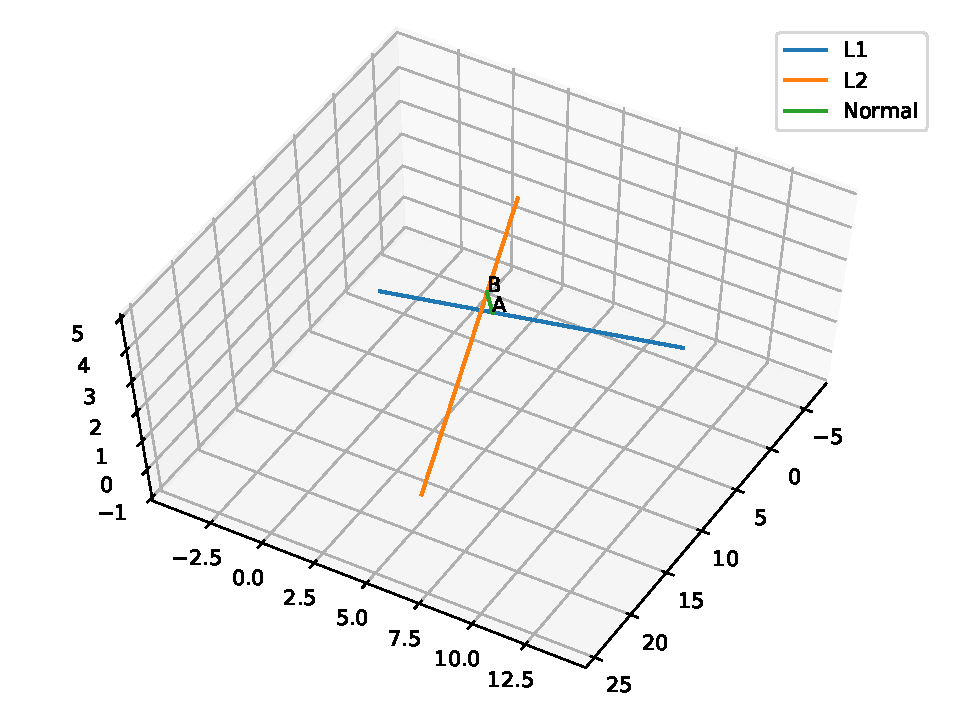
\includegraphics[width=\columnwidth]{figs/problem30.pdf}
	\end{center}
\caption{}
\label{fig:Fig1}
\end{figure}
\end{enumerate}
\end{document}
